%===============================================
\section{Measurement of Higgs boson couplings}
\frame{\tableofcontents[currentsection]}


%%=================================================================================
\begin{frame}{Methodology}
  \begin{minipage}{0.49\linewidth}
    For a given systematic source :
    \begin{itemize}
    \item Create distributions of \\ $m_{\gamma\gamma}^{nom}$, $m_{\gamma\gamma}^{up}$, $m_{\gamma \gamma}^{down}$
    \item Fit main parameter of the systematic with DSCB :
      \begin{itemize}
      \item Fit  $m_{\gamma\gamma}\in[105,160]$GeV
      \item Fixing $n_{high}=5$ and $n_{low}=9$
      \item Fixing $\alpha_{high}=\hat{\alpha}_{high}^{nom}$, $\alpha_{low}^{nom}=\hat{\alpha}_{low}^{nom}$, $X=\hat{X}^{nom}$
%        \item Fixing secondary parameter to nominal fitted values.
      \end{itemize}
      \item Systematic variation : $\frac{X^{fluct}}{X^{nom}}-1$, $X\in \{\mu , \sigma\}$
      \end{itemize}
    \end{minipage}
    \hfill
    \begin{minipage}{0.49\linewidth}
      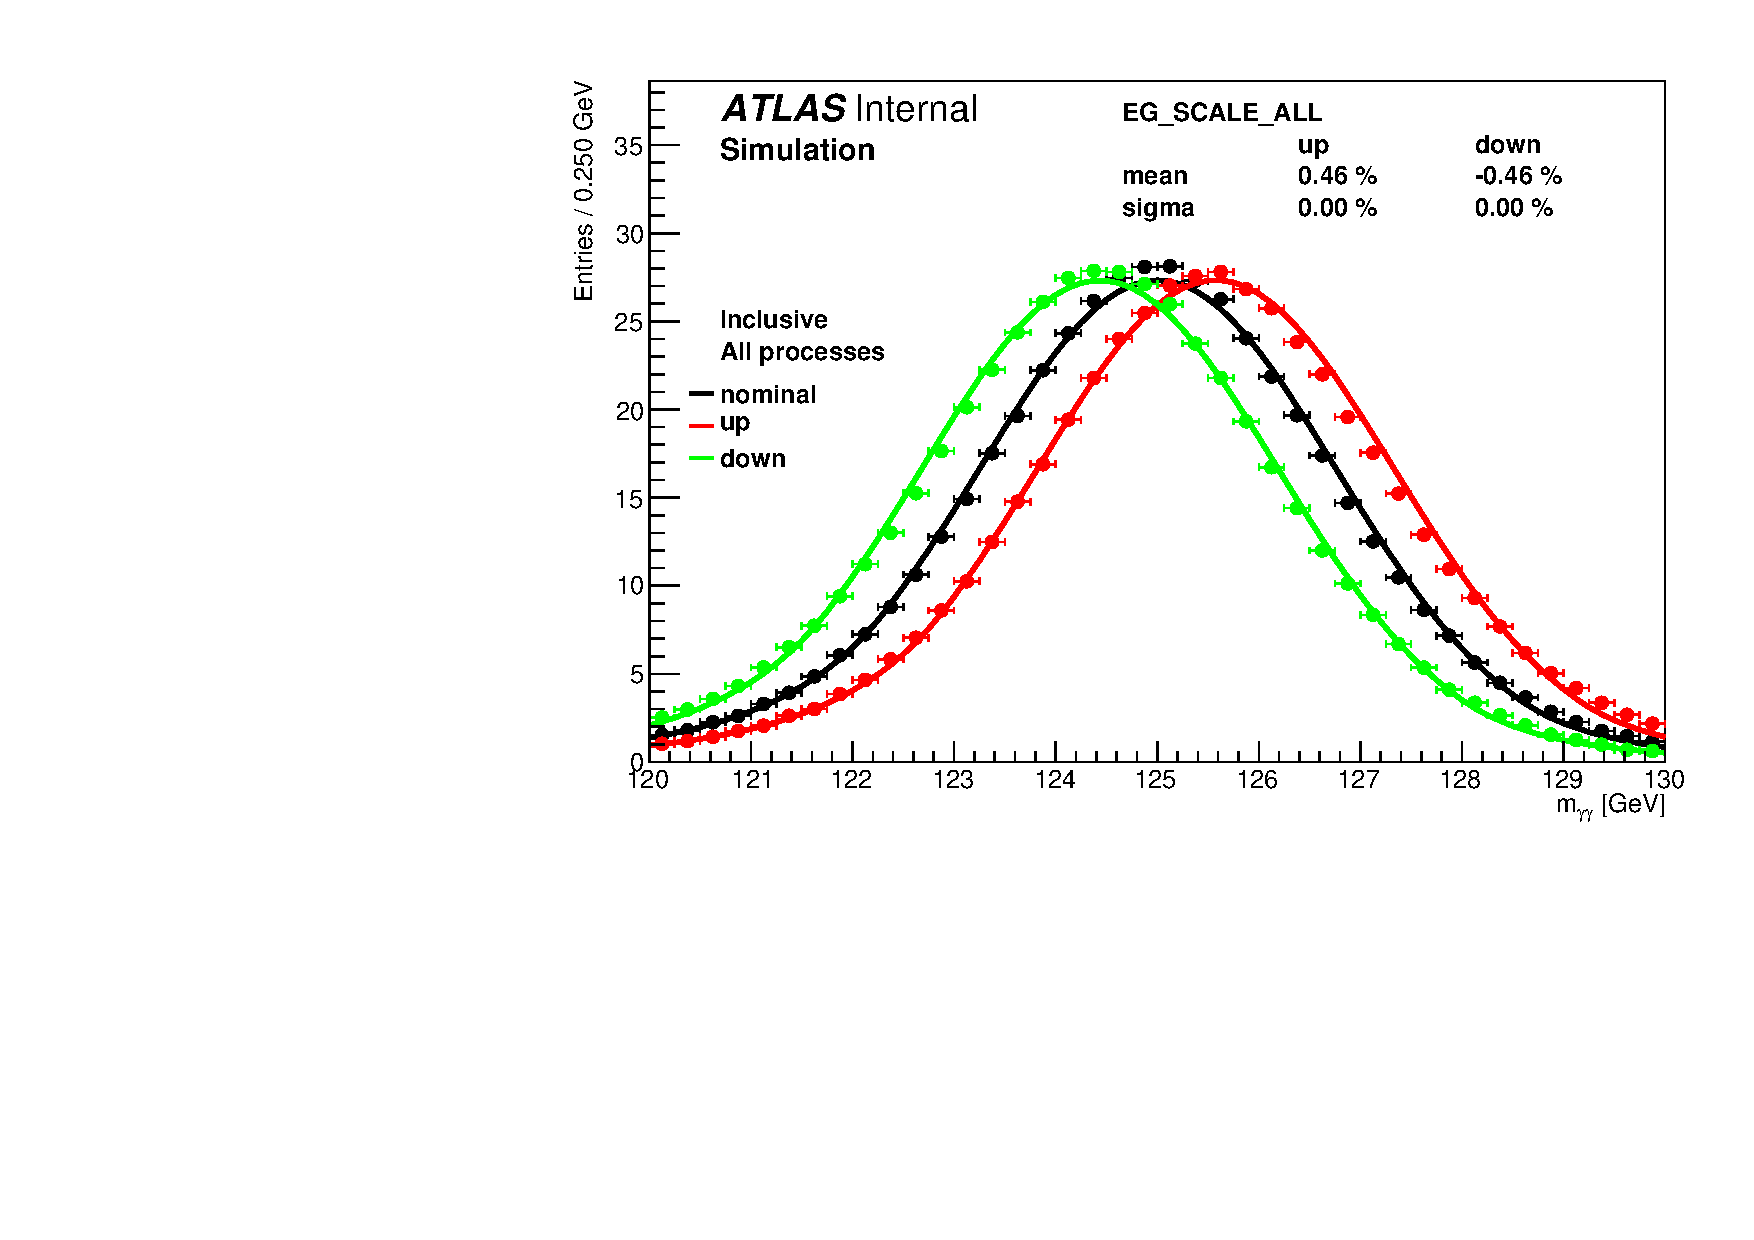
\includegraphics[width=\linewidth]{Figures/h013_EG_SCALE_ALL_0.pdf}
    \end{minipage}
    \vfill
    
    \begin{equation}
      \tiny
      CB(m_{\gamma \gamma}) = 
      \begin{cases}
        e^{-t^{2}/2} & \text{if } -\alpha_{low} \leq t \leq \alpha_{high} \\
        \frac{ e^{-{}^{1}_{2} \alpha_{low}^{2}} } { \left[ \frac{1}{R_{low}} \left(R_{low} - \alpha_{low} - t \right) \right]^{n_{low}} } & \text{if } t < -\alpha_{low} \\
        \frac{ e^{-{}^{1}_{2} \alpha_{high}^{2}} } { \left[ \frac{1}{R_{high}} \left(R_{high} - \alpha_{high} + t \right) \right]^{n_{high}} } & \text{if } t > \alpha_{high} \\
        t=(m_{\gamma\gamma}-\mu)/\sigma, R_{low}=\frac{\alpha_{low}}{n_{low}},  R_{high}=\frac{\alpha_{high}}{n_{high}} \\
      \end{cases}
    \end{equation}

%    More work required to improve fits quality.
\end{frame}

%%====================================================================
\begin{frame}{Likelihood Method}
A function ({\bf likelihood}) is built to {\bf evaluate the best set of parameters ($\vec{\mu}$,$\vec{\theta}$)} of a model to agree the best with a dataset in a category.

$$\mathcal{L}=\underbrace{\frac{(n_{s}(\vec{\mu},\vec{\theta})+b)^{n_{obs}}}{n_{obs}!} e^{-(n_{s}(\vec{\mu},\vec{\theta})+b)}}_{\textcolor{red}{\text{(1)}}}  \overbrace{\prod_j^{n_{obs}}\psi(\vec{x_j};\vec{\mu},\vec{\theta})}^{\textcolor{violet}{\text{(2)}}} \underbrace{e^{-\frac{\theta^2}{2}}}_{\textcolor{blue}{\text{(3)}}}$$
\vfill
\begin{minipage}{0.49\linewidth}
\textcolor{red}{(1) {\bf Poissonian law} to evaluate the probability to observe $n_{obs}$($\equiv$ signal $+$ background) events when $(n_s+b)$ are expected.}\newline
\textcolor{violet}{(2) {\bf Probability density function} of the observables $\vec{x}$ (diphoton invariant mass for example) for the $j^{th}$ event.}\newline
\textcolor{blue}{(3) Constraint on the nuisance parameter $\theta$. See next slide.}\newline
\end{minipage}
\begin{minipage}{0.49\linewidth}
\includegraphics[width=\linewidth]{Cgam_009.png}
\end{minipage}
\end{frame}


%%==========================================================

\begin{frame}{Nuisance parameters}
There are some {\bf external measurements}  that contribute to the likelihood and have some {\bf uncertainties}. 
A {\bf free nuisance parameter} is added for each of these measurements.
In order  to take into account these external measurements, a {\bf constraint is put on these nuisance parameters}. 
\vfill
For example, the luminosity is re-defined as  $L(1+\delta_L \theta_L)$, with $\theta_L$ the nuisance parameter and $\delta_L$ the uncertainty on the luminosity (assumed to be Gaussian).
In this case, a Gaussian constraint is chosen.

The contribution from luminosity will hence be :
$$L(1+\delta_L \theta_L)e^{-\theta_L^2/2}$$
\vfill
\textcolor{blue}{\bf Error Estimation}\newline
A test statistic is defined as : $t_\mu=-2ln\frac{\mathcal{L}(\mu,\hat{\hat{\theta}})}{\mathcal{L}(\hat{\mu},\hat{\theta})}$, with $\hat{\theta}$ and $\hat{\mu}$ the best (fitted) parameters, and $\hat{\hat{\theta}}$ the fitted nuisance parameters for a fixed $\mu$.\newline
Uncertainty are given by : \textcolor{red}{$\mathbf{t_{\hat{\mu}\pm 1\sigma}=1}$} and \textcolor{red}{$\mathbf{t_{\hat{\mu}\pm 2\sigma}=4}$} in 1D Gaussian limit.
\end{frame}

